

\documentclass[aos,noinfoline]{imsart} % annals of applied statistics 
\setattribute{journal}{name}{} 

\RequirePackage[OT1]{fontenc}
\RequirePackage{amsthm,amsmath,amssymb}
\RequirePackage[square,authoryear,sort]{natbib}
\RequirePackage[authoryear]{natbib}
\RequirePackage[colorlinks,citecolor=blue,urlcolor=blue]{hyperref}

% settings
%\pubyear{2014}
%\volume{0}
%\issue{0}
%\firstpage{1}
%\lastpage{8}
%\arxiv{arXiv:0000.0000}

\usepackage{macros}
%\usepackage{fullpage}
\usepackage[left=0.85in,right=0.85in, top=1.0in,bottom=0.75in]{geometry}
\usepackage[mathcal, mathscr]{eucal}
\usepackage{colortbl}
\usepackage[size=small]{caption}
\usepackage{subcaption}
\usepackage{graphicx}
\graphicspath{{./figures/}}
\DeclareGraphicsExtensions{.pdf,.png,.jpg}
\usepackage{algorithm}
\usepackage{algorithmic}
\usepackage[authoryear,sort]{natbib}
\setcitestyle{authoryear,square}
\usepackage{todonotes}

\bibpunct[; ]{(}{)}{;}{a}{,}{;} 


\usepackage{booktabs}

\newcommand{\vect}{\boldsymbol}
\newcommand{\matr}{\boldsymbol}
\newcommand{\diag}{\textrm{diag}}

\newcommand{\specialcell}[2][c]{%
  \begin{tabular}[#1]{@{}c@{}}#2\end{tabular}}
  
\endlocaldefs

\begin{document}

\begin{frontmatter}
\title{Discovering switching autoregressive dynamics in neural spike train recordings} 
%\runtitle{Learning semiparametric Hodgkin-Huxley models}
\begin{aug}

\author{\fnms{Scott W.} \snm{Linderman},\ead[label=e1]{swl@seas.harvard.edu}}
\author{\fnms{Matthew J.} \snm{Johnson},\ead[label=e2]{mattjj@mit.edu}}
\author{\fnms{Sandeep R.} \snm{Datta},\ead[label=e3]{srdatta@hms.harvard.edu}}
\and
\author{\fnms{Ryan P.} \snm{Adams}\ead[label=e4]{rpa@seas.harvard.edu}}
%\thankstext{t2}{Supported by the Center for Brains, Minds and Machines (CBMM)}
%\thankstext{t3}{Partially funded by NSF STC award CCF-1231216. }
\runauthor{S. W. Linderman, M. J. Johnson, S. R. Datta, and R. P. Adams}
%
\affiliation{Harvard University, Harvard Medical School} 

%\address{Scott W. Linderman\\
%School of Engineering and Applied Science \\
%Harvard University\\
%Cambridge, MA 02138,  USA\\
%\printead{e2}
%}
%
%\address{Aaron Tucker\\
%Harvard College\\
%Cambridge, MA 02138,  USA\\
%\printead{e1}
%}
%
%\address{Ryan P. Adams\\
%School of Engineering and Applied Science \\
%Harvard University\\
%Cambridge, MA 02138,  USA\\
%\printead{e3}
%}
\end{aug}

\end{frontmatter}

\section{Abstract} 
Generalized linear models (GLM) are powerful tools for identifying dependence in spiking populations of neurons, both over time and within the population \cite{Paninski-2004}.  The GLM identifies these dependencies by modeling spiking patterns through a linear regression and an appropriately-selected link function and likelihood.  This regression setup is appealing for its simplicity, the wide variety of available priors, the potential for interpretability, and its computational efficiency.  However, the GLM suffers from at least three notable deficiencies.  First, the model is linear up to the link function, which only allows a limited range of response maps from neural spiking histories.  Second, the model's parameters are fixed over time, while neural responses may vary due to processes that are exogenous to the population.  Third, the generalized linear model presupposes a characteristic time scale for all dynamics, when there may be multiple, varying time scales of neural activity in a given population. 

Here we seek to address these deficiencies via a \emph{switching} variant of the generalized linear model.  A switching system is one that evolves through a set of discrete states over time, with each state exhibiting its own low-level dynamics.  For example, the latent state of a hidden Markov model (HMM) can be used to determine the parameters of an autoregressive (AR) process.  These HMM-AR models can be used to identify common patterns of linear dependence that vary over time. Bayesian nonparametric versions of HMM-AR models extend these ideas to allow for an infinite number of such patterns to exist \emph{a priori}, and \emph{semi-Markov} variants allow the different states to have idiosyncratic duration distributions.  Here we develop GLM variants of these switching AR processes and specialize them for neural spiking data.  In particular, we exploit recent data augmentation schemes for negative binomial likelihood functions \cite{Pillow-2012} to make inference tractable in HDP-HSMM-AR models with count-based observations.

\section{Models}
The fundamental building block of our spike train models is a hidden Markov model~(HMM) consisting of~$K$ latent states, an initial state distribution~$\bpi$, and a stochastic transition matrix~${\bA\in [0,1]^{K\times K}}$. The probability of transitioning from state~$k$ to state~$k'$ is given by entry~${A_{k,k'}}$. The latent state in the~$t$-th time bin is given by~${z_t\in\{1,\ldots,K\}}$. We observe a sequence of vectors~${\bs_t\in\naturals^N}$ where~$s_{n,t}$ specifies the number of spikes emitted by the~$n$-th neuron during the~$t$-th time bin. 

To model autoregressive structure in the spike train, we model the spike count vectors~$\bx_t$ as arising from an autoregressive negative binomial model. The expected number of spikes is a weighted function of recent spike count vectors. Specifically, let 
\begin{align}
\bpsi_{n} \sim \distNormal(\bmu_{\bpsi}, \sigma_{\bpsi}^2 \bI),
\quad
\bmu_{\bpsi} = \bX \bw_{n}^{(k)},
\end{align}
where~${\bX\in \reals^{T\times B}}$ is a matrix of given regressors and ${\bw_{n}^{(k)}\in \reals^B}$ is a vector of weights specific to neuron~$n$ and the~$k$-th latent state. Typically the regressors include the filtered spike history and externally applied stimuli, allowing the weights to be interpreted as ``functional interaction'' strengths and stimulus response functions. Let~${\bW^{(k)}=\{\bw_1^{(k)},\ldots,\bw_N^{(k)}\}}$ denote the set of all weight vectors for state~$k$. This model allows the weights to vary over time with the latent state of the population.

Together these specify a joint probability distribution,
\begin{align*}
p(\{\bs_t, z_t\}_{t=1}^T \given \bpi, \bA, \{\bW^{(k)}\}_{k=1}^K, \bX, \xi, \sigma_{\bpsi}^2) &= p(z_1\given \bpi) \prod_{t=2}^T p(z_t \given z_{t-1}, \bA) \prod_{t=1}^T p(\bs_t \given z_t, \{\bW^{(k)}\}_{k=1}^K, \bX, \xi, \sigma_{\bpsi}^2),\\
p(z_1 \given \bpi) = \text{Multinomial}(z_1 \given \bpi), &\qquad p(z_t \given z_{t-1}, \bA) = \text{Multinomial}(z_t \given \bA_{z_{t-1},:}),
\end{align*}
and
\begin{align*}
p(\bpsi_t \given z_t, \bX, \{\bW^{(k)}\}_{k=1}^K) &= \prod_{n=1}^N \distNormal(\psi_{n,t} \given \bX\bw_{n}^{(z_t)}, \sigma_{\bpsi}^2), \\
p(\bs_t \given \bpsi_t, \xi) &= \prod_{n=1}^N \text{NegBin}(s_{n,t} \given \xi, \sigma(\psi_{n,t})),
\end{align*}
where~$\sigma(\cdot)$ denotes the logistic function. 
We use a hierarchical Dirichlet process (HDP) as a prior distribution on the rows of the transition matrix, thereby allowing for nonparametric inference of the number of states.  Additionally, we consider a hidden semi-Markov model (HSMM). In a standard HMM, the amount of time spent in state~$k$ is geometrically distributed as a function of~$A_{k,k}$. In many real-world examples, however, the state durations may follow more interesting distributions. As with the HMM, we can also derive a nonparametric extension called the HDP-HSMM with similarly efficient inference algorithms. 


\begin{figure}[t!]
  \centering%
  \begin{subfigure}[T]{1.2in}
    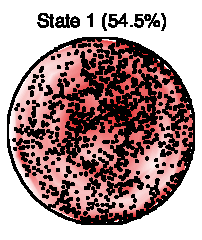
\includegraphics[width=\textwidth]{state1}
  \end{subfigure}
  ~
  \begin{subfigure}[T]{1.2in}
    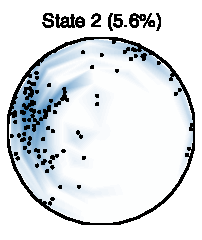
\includegraphics[width=\textwidth]{state2}
  \end{subfigure}
  ~
  \begin{subfigure}[T]{1.2in}
    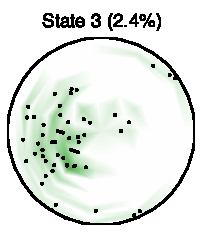
\includegraphics[width=\textwidth]{state3}
  \end{subfigure}
    ~
  \begin{subfigure}[T]{1.2in}
    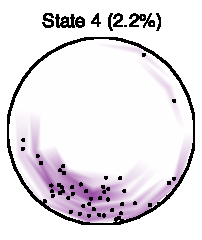
\includegraphics[width=\textwidth]{state4}
  \end{subfigure}
    ~
  \begin{subfigure}[T]{1.2in}
    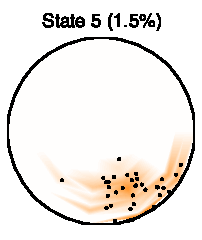
\includegraphics[width=\textwidth]{state5}
  \end{subfigure}
  \\
  % Networks
    \begin{subfigure}[T]{1.2in}
    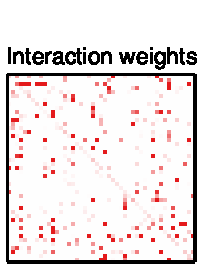
\includegraphics[width=\textwidth]{network1}
  \end{subfigure}
  ~
  \begin{subfigure}[T]{1.2in}
    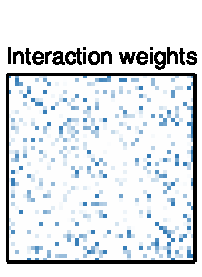
\includegraphics[width=\textwidth]{network2}
  \end{subfigure}
  ~
  \begin{subfigure}[T]{1.2in}
    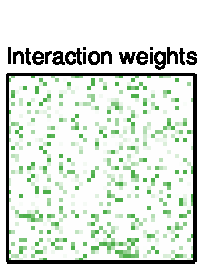
\includegraphics[width=\textwidth]{network3}
  \end{subfigure}
    ~
  \begin{subfigure}[T]{1.2in}
    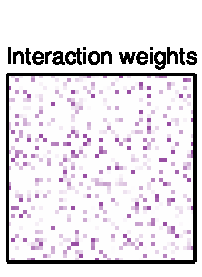
\includegraphics[width=\textwidth]{network4}
  \end{subfigure}
    ~
  \begin{subfigure}[T]{1.2in}
    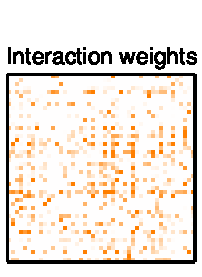
\includegraphics[width=\textwidth]{network5}
  \end{subfigure}
\vspace{-.5em}
\caption{A sample of five inferred latent states in a 9 minute recording of hippocampal place cells from a rat exploring a circular arena. The spike counts are modeled as negative binomial distributed with parameters that depend upon previous spike history. The top row shows the distribution of locations of the rat corresponding to each of the inferred states. The bottom row shows the functional network of interaction weights (~$||\bW^{(k)}||_1$, a~$38\times 38$ matrix) corresponding to each latent state.}
\label{fig:figure1}

\end{figure}

\section{Results}
We applied the switching GLM to a 9 minute recording of hippocampal place cells from a rat exploring a circular arena 1 meter in diameter, courtesy of Prof. Matthew Wilson's lab at MIT. 38 neurons are identified, and spikes are counted in 250ms time bins. We used the previous four bins (1 second) of spike history as regressors. Thus, the weights of the model can be interpreted as interaction weights between pairs of neurons. Figure~\ref{fig:figure1} shows five of the inferred latent states, the spatial location of the rat while in each inferred state, and the~$N\times N$ network of interaction weights for each pair of neuron. To reduce the regression weights to a scalar, we take the~$L_1$ norm of the weight vector for each functional weight vector. In this case, we have inferred that the spike counts are well-modeled by latent states that correspond to different networks of functional interaction in the different regions of the arena.  In future work, we hope to delve into these latent states in more detail and identify the properties that differentiate one state from another.  

\bibliographystyle{imsart-nameyear}
{\small \bibliography{draft}}

\clearpage

\end{document}

   
